\documentclass[main.tex]{subfiles}
\begin{document}

\chapter{Examens}
\label{cha:examens}
In dit hoofstuk worden oude examens opgelost.
Er wordt telkens eerst de opgave gegeven en daarna de oplossing.
Merk op dat de opgaven gratis online beschikbaar zijn.
Let ook op, de examenvragen komen hoogstwaarschijnlijk niet terug, maar het zijn goede oefeningen.


\includepdf[pages=-]{opgaven/januari_2012_1.pdf}

\section{Januari 2012 I}

\subsection*{Mondeling gedeelte}
\begin{enumerate}
\item
  \begin{enumerate}[(a)]
  \item Zie definitie \ref{de:spiegeling} op pagina \pageref{de:spiegeling}
  \item Zie stelling \ref{st:spiegeling-isometrie} op pagina \pageref{st:spiegeling-isometrie}
  \item Een spiegeling om een $m$-dimensionale affiene deelruimte in een $n$-dimensionale affiene deelruimte is ori\"entatiebewarend als en slecht als $n+m$ even is.
    \begin{figure}[H]
      \centering
      \begin{tabular}{|c|c|c|c|c|}
        \hline
        Spiegeling om $\downarrow$ in $\rightarrow$& $0D$ & $1D$ & $2D$ & $3D$\\\hline\hline
        punt & Bewarend & Omkerend & Bewarend & Omkerend\\\hline
        rechte & N/A & Bewarend & Omkerend & Bewarend\\\hline
        vlak & N/A & N/A & Bewarend & Omkerend \\\hline
        ruimte & N/A & N/A & N/A & Bewarend\\\hline
      \end{tabular}
      \caption{Spiegelingen}
    \end{figure}

  \end{enumerate}
\item \TODO{}
\end{enumerate}
\subsection*{Schriftelijk gedeelte}
\begin{enumerate}
\item
  \begin{enumerate}[(a)]
  \item 
    \[
    \begin{pmatrix}
      2\\0\\1\\1
    \end{pmatrix}
    + \lambda
    \begin{pmatrix}
      1\\2\\0\\2
    \end{pmatrix}
    =
    \begin{pmatrix}
      -1\\0\\4\\-5
    \end{pmatrix}
    + \mu
    \begin{pmatrix}
      2\\0\\1\\2
    \end{pmatrix}
    \longleftrightarrow
    \begin{pmatrix}
      3\\0\\-3\\-4
    \end{pmatrix}
    =
    \lambda
    \begin{pmatrix}
      -1\\-2\\-0\\-2
    \end{pmatrix}
    + \mu
    \begin{pmatrix}
      2\\0\\1\\2
    \end{pmatrix}
    \]
    \[
    \left(
      \begin{array}{cc|c}
        -1 & 2 & 3\\
        2 & 0 & 0\\
        0 & 1 & -3\\
        -2 & 2 & -4
      \end{array}
    \right)
    \]
    Dit stelsel is strijdig, dus de doorsnede van $L_{1}$ en $L_{2}$ is leeg.
    $(1,2,0,2)$ is bovendien lineair onafhankelijk van $(2,0,1,2)$, dus de rechten kruisen.
  \item 
    We kennen de richting van de gemeenschappelijke loodlijn kennen we nu al, we berekenen dus nog het snijpunt ervan met $L_{1}$.
    \[ 
    \begin{pmatrix}
      2\\0\\1\\1
    \end{pmatrix}
    + a
    \begin{pmatrix}
      1\\2\\0\\2
    \end{pmatrix}
    =
    \begin{pmatrix}
      -1\\0\\4\\-5
    \end{pmatrix}
    + b
    \begin{pmatrix}
      2\\0\\1\\2
    \end{pmatrix}
    + c
    \begin{pmatrix}
      0\\1\\2\\-1
    \end{pmatrix}
    \longleftrightarrow
    \begin{pmatrix}
      2 & 0 & 1 & 3\\
      0 & 1 & 2 & 0\\
      1 & 2 & 0 & -3\\
      2 & -1 & 2 & 6
    \end{pmatrix}
    \]
    De oplossing hiervan is $(a,b,c)=(1,-2,1)$.
    Het snijpunt van $L_{1}$ met de gemeenschappelijke loodlijn is dus $p$:
    \[
    \begin{pmatrix}
      2\\0\\1\\1
    \end{pmatrix}
    +
    \begin{pmatrix}
      1\\2\\0\\2
    \end{pmatrix}
    =
    \begin{pmatrix}
      3\\2\\1\\3
    \end{pmatrix}
    \]
    De gemeenschappelijke loodlijn is dan $L_{3}$:
    \[
    L_{3} =
    \begin{pmatrix}
      3\\2\\1\\3
    \end{pmatrix}
    +
    \lambda
    \begin{pmatrix}
      0\\1\\2\\-1
    \end{pmatrix}
    \]
  \item Nee, de richtingsvector van de gemeenschappelijke loodlijn moet van een zeer specifieke vorm zijn.
    % Elke vector op de gemeenschappelijke loodlijn van $S$ en $T$ staat loodrecht op zowel $(1,2,0,2)$ als $(2,0,1,2)$:
    % \[
    % \left\{
    %   \begin{array}{c}
    %     (1,2,0,2) \cdot (u,x,y,z) = 0\\
    %     (2,0,1,2) \cdot (u,x,y,z) = 0
    %   \end{array}
    % \right.
    % \longleftrightarrow
    % \left\{
    %   \begin{array}{c}
    %     u+2x+2z = 0\\
    %     2u+y+z = 0
    %   \end{array}
    % \right.
    % \longleftrightarrow
    % \begin{pmatrix}
    %   1 & 0 & \frac{1}{2} & 1\\
    %   0 & 1 & -\frac{1}{2} & 1
    % \end{pmatrix}
    % \]
  \end{enumerate}

\item 
  \begin{figure}[H]
    \centering
    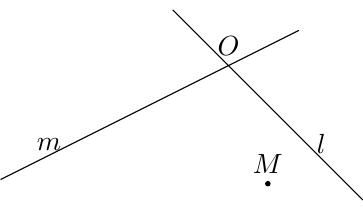
\begin{tikzpicture}[scale=1,extended line/.style={shorten >=-#1,shorten <=-#1},extended line/.default=1cm] 
      \coordinate [label=above:$O$] (o) at (1,2);
      \coordinate [label=left:$m$] (m1) at (-1,1);
      \coordinate [label=right:$l$] (l1) at (2,1);

      \draw [extended line=1cm] (o) -- (m1);
      \draw [extended line=1cm] (o) -- (l1);

      \coordinate [label=above:$M$] (m) at (1.5,.5);
      \fill (m) circle [radius=1pt];

    \end{tikzpicture}
  \end{figure}
  We zoeken een punt $A$ op $l$ en een punt $B$ op $m$ zodat $|AM|$ gelijk is aan $|MB|$ en $A$, $B$ en $M$ colineair zijn.
  Met andere woorden zodat $(A,B,M)$ gelijk is aan $1$.
  \[ M = \frac{1}{2}A + \frac{1}{2}B \]
  Noem het snijpunt van $l$ en $m$ $O$.
  \begin{itemize}
  \item Syntetisch\\
  \item \TODO{}
  \item Analytisch\\
  \item \TODO{}
  \item \TODO{}
  \end{itemize}
\item \TODO{}
\item \TODO{}
\end{enumerate}



\section{Januari 2012 II}

\includepdf[pages=-]{opgaven/januari_2012_2.pdf}






\includepdf[pages=-]{opgaven/januari_2011_1.pdf}

\includepdf[pages=-]{opgaven/januari_2011_2.pdf}

\includepdf[pages=-]{opgaven/augustus_2011.pdf}




\includepdf[pages=-]{opgaven/januari_2009_2.pdf}

\end{document}
